% !TeX spellcheck = en_GB

\section{Algorithms}\label{algorithms}

\subsection{Help Data Structure Pyramid and Others}

\noindent Define $[i,\ j]$: \\
$[i,\ j] := \{i,\ i+1,..., j-1,\ j\} \subseteq \mathbb{N}_{\geq 0}$.\\

\noindent Define $Pyramid$:\\
$Pyramid :=\{ cell_{i,j}\ |\ i \in \mathbb{N}_{\geq 0},\  j \in [0,\ j_{max}-i],\ i_{max} = j_{max} = |word|-1\}$.\\
$cell_{i,j} = \{c\ |\ c \subseteq V\}$.\\
$EmptyPyramid \Leftrightarrow \forall i\ \forall j\ cell_{i,j}=\emptyset$.\\
Regarding one $cell_{i,j}$: $cell_{i,j} = cellDown$, $cell_{i-1,j} = cellUpperLeft$ and $cell_{i-1,j+1} = cellUpperRight$  \\

\begin{figure}[h]
	\centering
	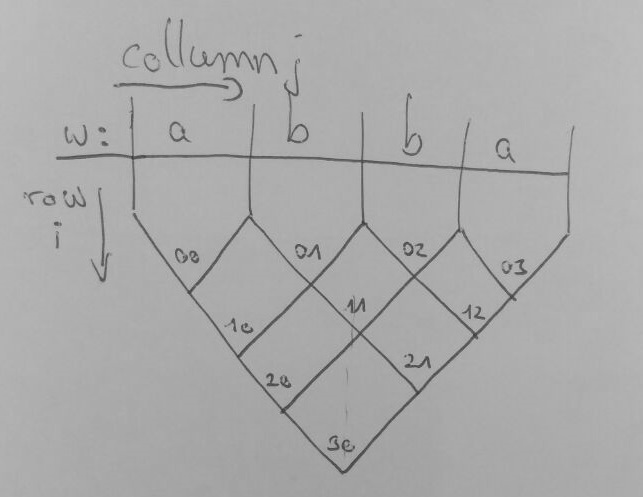
\includegraphics[width=0.7\textwidth]{abb/DataStructurePyramid}
\end{figure}

\pagebreak
\subsection{Exam Exercise Generating Algorithms}

\pagebreak

\subsubsection{Algorithm: AlgorithmName}

\paragraph{Basic Idea}

\paragraph{Tweak Idea 1 for Algorithm}

\paragraph{Tweak Idea 2 for Algorithm}

\paragraph{Finished Algorithm}



\pagebreak

\subsubsection{Algorithm: GeneratorGrammarDiceRollOnly}
\noindent Very naive way of generating grammars. This is intended to be our starting point for our algorithms we find. Each found algorithm must have a higher score that this algorithm or otherwise it would be worse than simple dice rolling. \\

\noindent
\frame{
	\begin{algorithm}[H] %or another one check
\caption{GeneratorGrammarDiceRollOnly}
\label{GeneratorGrammarDiceRollOnly}
\SetAlgoLined
\KwIn{ $Word\ w \in \Sigma^{*},\ P \subseteq V \times (V^{2} \cup \Sigma) = \emptyset,\ $ }
\KwOut{$Grammar\ G\ in\ CNF$}

$P = P \cup \{distribute\ \{\sigma\ |\ \sigma \in w \}\ over\ \{v\ |\ v \in V \} \} $\;
$P = P \cup \{distribute\ \{vc\ |\ vc \in V^2 \}\ $$over\ \{v\ |\ v \in V \} \} $\;
$P = P \setminus \{p\ |\ p \subseteq P,\ vc\ is\ right\ in\ p,\ \forall i\ \forall j\ vc \notin cell_{i,j}\ of\ the\ pyramid \} $\;
\Return $G$\;
	\end{algorithm}
}
\\
\\
\noindent
\frame{
	\begin{algorithm}[H] %or another one check
		\caption{GeneratorGrammarDiceRollOnlyBias}
		\label{GeneratorGrammarDiceRollOnlyBias}
		\SetAlgoLined
		\KwIn{ $Word\ w \in \Sigma^{*},\ P \subseteq V \times (V^{2} \cup \Sigma) = \emptyset,\ $ }
		\KwOut{$Grammar\ G\ in\ CNF$}
		
		NOT FINISHED, MAYBE LATER.\\		
		$pick\ uniform\ randomly\  \{v\ |\ v \in V\} with...\ $\;
		$...$\;
		$P = P \cup \{distribute\ \{\sigma\ |\ \sigma \in w \}\ over\ \{v\ |\ v \in V \} \} $\;
		$P = P \cup \{distribute\ \{vc\ |\ vc \in V^2 \}\ $$over\ \{v\ |\ v \in V \} \} $\;
		$P = P \setminus \{p\ |\ p \subseteq P,\ vc\ is\ right\ in\ p,\ \forall i\ \forall j\ vc \notin cell_{i,j}\ of\ the\ pyramid \} $\;
		\Return $G$\;
	\end{algorithm}
}

\pagebreak
\subsubsection{Algorithm: BottomUp GeneratorGrammarDiceRollMartens1}
\noindent Things like the $G=(V,\Sigma , S, P)$ can be assumed as known.\\
$P = P \cup \{distribute\ \{\sigma\ |\ \sigma \in w \}\ uniform\ randomly\ over\ \{v\ |\ v \in V \} \}$ which equals $distributeRhse$ method.\\
\noindent Bias is only allowed top vs down regarding the pyramid. No left or right bias intended yet.\\

\noindent
\frame{
	\begin{algorithm}[H] %or another one check
		\caption{GeneratorGrammarDiceRollMartens}
		\label{GeneratorGrammarDiceRollMartens}
		\SetAlgoLined
		\KwIn{ $Word\ w \in \Sigma^{*},\ P \subseteq V \times (V^{2} \cup \Sigma) = \emptyset,\ $ }
		\KwOut{$Grammar\ G\ in\ CNF$}
		
		$P = P \cup \{distribute\ \{\sigma\ |\ \sigma \in w \}\ over\ \{v\ |\ v \in V \} \} $\;
		$pyramid = CYK(G,\ w)$\;
		\For{$i:=1\ \textbf{to}\ i_{max}$}{
			$J \subseteq \mathbb{N} = \emptyset $\;
			$cellSet \subseteq V^2= \emptyset$\;
			\While{$|J| < j_{max}-i$}{
				$choose\ one\ j \notin J\ uniform\ randomly\ in\ [0, j_{max}-i] $\;
				$J = J \cup j$\;
				$cellSet = calculateSubsetForCell(pyramid,\ i,\ j)$\;
				$P = P \cup \{distribute\ \{vc\ |\ vc \in cellSet \}\ $$over\ \{v\ |\ v \in V \} \} $\;
				$pyramid = CYK(G,\ w)$\;	
				$evaluate\ stopping\ criteria\ regarding\ the\ pyramid$\;
				\If{$stopping\ criteria = true$}{
					\Return $G$\;
				}
			}
		}
		\Return $G$\;
		\footnotetext{
			\noindent Line 2: Fills the i=0 row of the pyramid.
			
			\noindent Line 4: Instead of going from left to right, choose $j$ uniform randomly with the restrictions that one cell is only visited one time.
			
			\noindent Note: Maybe modify algorithm to also work with the threshold.
		}
	\end{algorithm}
}

\pagebreak
\subsubsection{Algorithm: BottomUp GeneratorGrammarDiceRollMartens2}
\noindent
\frame{
	\begin{algorithm}[H] %or another one check
		\caption{GeneratorGrammarDiceRollMartens2}
		\label{GeneratorGrammarDiceRollMartens2}
		\SetAlgoLined
		\KwIn{ $Word\ w \in \Sigma^{*},\ P \subseteq V \times (V^{2} \cup \Sigma) = \emptyset,\ $ }
		\KwOut{$Grammar\ G\ in\ CNF$}
		$P = P \cup \{distribute\ \{\sigma\ |\ \sigma \in w \}\ over\ \{v\ |\ v \in V \} \} $\;
		$pyramid = CYK(G,\ word)$\;
		%		$rowSet \subseteq V^2 \times \mathbb{N}  = \emptyset$\;
		\For{$i:=1\ \textbf{to}\ i_{max}$}{
			%$choose\ j\ uniform\ randomly\ in\ [0,\ j_{max}-i]  $\;
			\For{$j:=0\ \textbf{to}\ j_{max}-i$}{
				$rowSet = rowSet \cup \{(XY,i)\ |\ X,Y \in V,\ $ $XY \in calculateSubsetForCell(Pyramid,\ i,\ j) \}$\;
			}
			\While{$threshold_i = false $}{
				$choose\ one\ vc \in rowSet\ with\ priority,\ depending\ on\ i,\ $ $ uniform\ randomly$\;
				$P = P \cup \{distribute\ \{vc\ |\ vc \in cellSet \}\ $$over\ \{v\ |\ v \in V \} \} $\;
				$pyramid = CYK(G,\ w)$\;
				$evaluate\ and\ update\ threshold_i,\ regarding\ line\ i$\;
				$evaluate\ stopping\ criteria,\ regarding\ the\ pyramid$\;
				\If{$stopping\ criteria = true$}{
					\Return $G$\;
				}	
			}
		}
		\Return $G$\;
		\footnotetext{
			\noindent Line 2: Fills the i=0 row of the pyramid.
			
			\noindent Line 6: $(AB,1), (AB,2), (BC,3) ... \in sub$ $\rightarrow$ multiple occurrences of $AB$ are allowed. This considers "more important" compound variables. 
			
			\noindent Line 9: One vc can be chosen several times.
			
			\noindent Note: Threshold: Linear or log function $f(i)$?
			
			\noindent Note: Priority mechanism: In line $i+1$ the $k = \{(A,l)\ |\ (A,l) \in sub,\ l=i  \}$ are preferred over the\\ $m = \{(A,n)\ |\ (A,n) \in sub,\ n < i  \}$. In what way are they preferred? Using some kind of factor to weight the $i$ of $(A,i)$.
		}
	\end{algorithm}
}
\pagebreak 
\subsubsection{Algorithm: TopDown From node to leaves}
\subsubsection{Algorithm: How often cells are used for subset calculations}

\pagebreak

\subsubsection{Tweaking Sub Procedures in more detail}
Maybe don't keep this so that the Algorithms can be read without flipping pages.\\

\noindent
\frame{
	\begin{algorithm}[H] %or another one check
		\caption{distributeRhse2}
		\label{distributeRhse2}
		\SetAlgoLined
		\KwIn{ $Rhse \subseteq\ (V^{2} \cup \Sigma),\ i \in  \mathbb{N},\ j \in  \mathbb{N}$}
		\KwOut{$Grammar\ G\ in\ CNF\ with\ uniform\ randomly\ distributed\ Rhse's.$}
		$choose\ n\ uniform\ randomly\ in\ [i, j]$\;
		$choose\ V_{add} := uniform\ random\ subset\ of\ size\ n\ from\ V$\;
		$P = P \cup \{ "v \longrightarrow rhse"\ |\ v \in V_{add},\ rhse \in Rhse \} $\;	
		
		\Return $G$;
	\end{algorithm}
}
Algorithm \ref{distributeRhse2} isn't needed anymore for the descriptions of the basic idea of the algorithm. It will be a module later on while tweaking the algorithms.
\\
\\
\frame{
	\begin{algorithm}[H] %or another one check
		\caption{calculateSubsetForCell}
		\label{calculateSubsetForCell}
		\SetAlgoLined
		\KwIn{$cell_ {i,j} \in pyramid $}
		\KwOut{$V_{i,j} \subseteq V^2$}
		$V_{i,j} = \emptyset $\;
		\For{$m:=i-1 \to 0$}{
			$V_{i,j} = V_{i,j} \cup \{X\ |\ X\longrightarrow YZ,\ Y \in V_{m,j},\ Z \in V_{i-m-1,m+j+1} \}$\;
		}
		
		\Return $V_{i,j}$;
	\end{algorithm}
}
Algorithm \ref{calculateSubsetForCell} describes the magic of the CKY-algorithm. It shows what cells are taken into account while filling one cell of the parse table.

\pagebreak

\subsection{Criteria Checking Procedures}
\noindent Description of the checks here. \\
\noindent All test of the GrammarValidityChecker class are based on the simple setV matrix. \\

\noindent  isValid = isWordProducible \&\& isExamConstraints \&\& isGrammarRestrictions\\

\noindent  isWordProducible = CYK.algorithmAdvanced()\\

\noindent  isExamConstraints = isRightCellCombinationsForced \&\& isMaxSumOfProductionsCount \&\& isMaxSumOfVarsInPyramidCount \&\& countRightCellCombinationsForced \\

\noindent isGrammarRestrictions = isSizeOfWordCount \&\& isMaxNumberOfVarsPerCellCount \\
\\
\\
\noindent 
\frame{
	\begin{algorithm}[H] %or another one check
		\caption{checkForceCombinationPerCell}
		\label{checkRightCellPerCombination}
		\SetAlgoLined
		\KwIn{$ cell_{i,j}\subseteq V,\ cell_{i-1,j}\subseteq V,\ cell_{i-1,j+1} \subseteq V,\ P \subseteq V \times (V^{2} \cup \Sigma) $ }
		\KwOut{$varsForcing \subseteq V$}
		$varsForcing \subseteq V = \emptyset$\;
		$varComp = \{XY\ |\ X \in cell_{i-1,j}\ \wedge\ Y \in cell_{i-1,j+1} \}$\;
		\ForEach{$v \in cell_{i,j}$}{
			$prods = \{p\ |\ p \subseteq P,\ v\ is\ left\ in\ p \}$\;
			$rhses = \{rhse\ |\ rhse\ is\ right\ in\ p \in prods\} $\;
			\If{$varComp \nsubseteq rhses$}{
				$varsForcing = varsForcing \cup v$\;
			}			
		}
		\Return $varsForcing$\;
		\footnotetext{Input: $cell_{i,j} = cellDown$, $cell_{i-1,j} = cellUpperLeft$ and $cell_{i-1,j+1} = cellUpperRight$
		}
	\end{algorithm}
}
Algorithm \ref{checkRightCellPerCombination} is a check that needs to be explained.
\\
\\
\frame{
	\begin{algorithm}[H] %or another one check
		\caption{checksumOfProductions}
		\label{checksumOfProductions}
		\SetAlgoLined
		\KwIn{$ max \in \mathbb{N}_{\geq 0}  $ }
		\KwOut{$ true \iff sum \leq max$}
		\If{$|P| > max $}{
			\Return $fales$\;
		}
		\Return $true$\;
	\end{algorithm}
}
Algorithm \ref{checksumOfProductions} can be explained via the Output of the algorithm alone.

\pagebreak

\noindent
\frame{
	\begin{algorithm}[H] %or another one check
		\caption{checkMaxNumberOfVarsPerCell}
		\label{checkMaxNumberOfVarsPerCell}
		\SetAlgoLined
		\KwIn{$ max \in \mathbb{N}_{\geq 0}  $ }
		\KwOut{$ true \iff \forall cell_{i,j} \in pyramid,\ |cell_{i,j}| \leq max $}
		\For{$i:=1\ \textbf{to}\ i_{max}$}{
			%$choose\ j\ uniform\ randomly\ in\ [0,\ j_{max}-i]  $\;
			\For{$j:=0\ \textbf{to}\ j_{max}-i$}{
				\If{$|cell_{i,j}| > max$}{
					\Return $false$\;
				}
			}
		}
		\Return $true$\;
	\end{algorithm}
}
Algorithm \ref{checkMaxNumberOfVarsPerCell} can be explained via the Output of the algorithm alone.
\\
\\
\noindent
\frame{
	\begin{algorithm}[H] %or another one check
		\caption{checkMaxSumOfVarsInPyramid}
		\label{checkMaxSumOfVarsInPyramid}
		\SetAlgoLined
		\KwIn{$ max \in \mathbb{N}_{\geq 0}  $ }
		\KwOut{$ true \iff sum \leq max $}
		$sum = 0$\;
		\For{$i:=1\ \textbf{to}\ i_{max}$}{
			%$choose\ j\ uniform\ randomly\ in\ [0,\ j_{max}-i]  $\;
			\For{$j:=0\ \textbf{to}\ j_{max}-i$}{
				$sum = sum + |cell_{i,j}|$\;
				\If{$sum > max$}{
					\Return $false$\;
				}
			}
		}
		\Return $true$\;
	\end{algorithm}
}
Algorithm \ref{checkMaxSumOfVarsInPyramid} could possible be explained via a simple mathematical statement like the algorithms \ref{checksumOfProductions} and \ref{checkMaxNumberOfVarsPerCell}.

\pagebreak